% Exercise ID: MAT_A12OTIMI_PROB_RAM_001
% Module: Módulo A12 - Otimização | Concept: Problemas Simples de Otimização
% Type: problemas_de_rampas | Difficulty: 2/5
% Tags: trigonometria, rampas, acessibilidade, angulo
% Author: Professor | Date: 2025-11-25

\exercicio{
Uma rampa de acesso para cadeiras de rodas tem 4 metros de comprimento horizontal e sobe 30 centímetros de altura.

\begin{center}
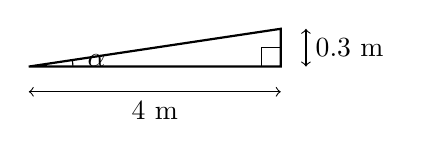
\begin{tikzpicture}[scale=0.8]
    \draw[thick] (0,0) -- (4,0) -- (4,0.6) -- cycle;
    \draw (3.7,0) rectangle (4,0.3);
    \draw[<->] (0,-0.4) -- (4,-0.4) node[midway,below] {4 m};
    \draw[<->] (4.4,0) -- (4.4,0.6) node[midway,right] {0.3 m};
    \draw (0.7,0) arc (0:8.5:0.7) node[right,xshift=2pt] {$\alpha$};
\end{tikzpicture}
\end{center}
}

\subexercicio{Converte a altura para metros.}

\subexercicio{Usa a razão trigonométrica adequada para calcular $\tan(\alpha)$.}

\subexercicio{Calcula o ângulo $\alpha$ (em graus). Usa a calculadora para encontrar $\tan^{-1}$ (arctangente).}

\subexercicio{As normas de acessibilidade recomendam um ângulo máximo de 5°. Esta rampa cumpre a norma? Justifica.}
